\begin{figure}[!h]
\centering
\resizebox{\textwidth}{!}{%
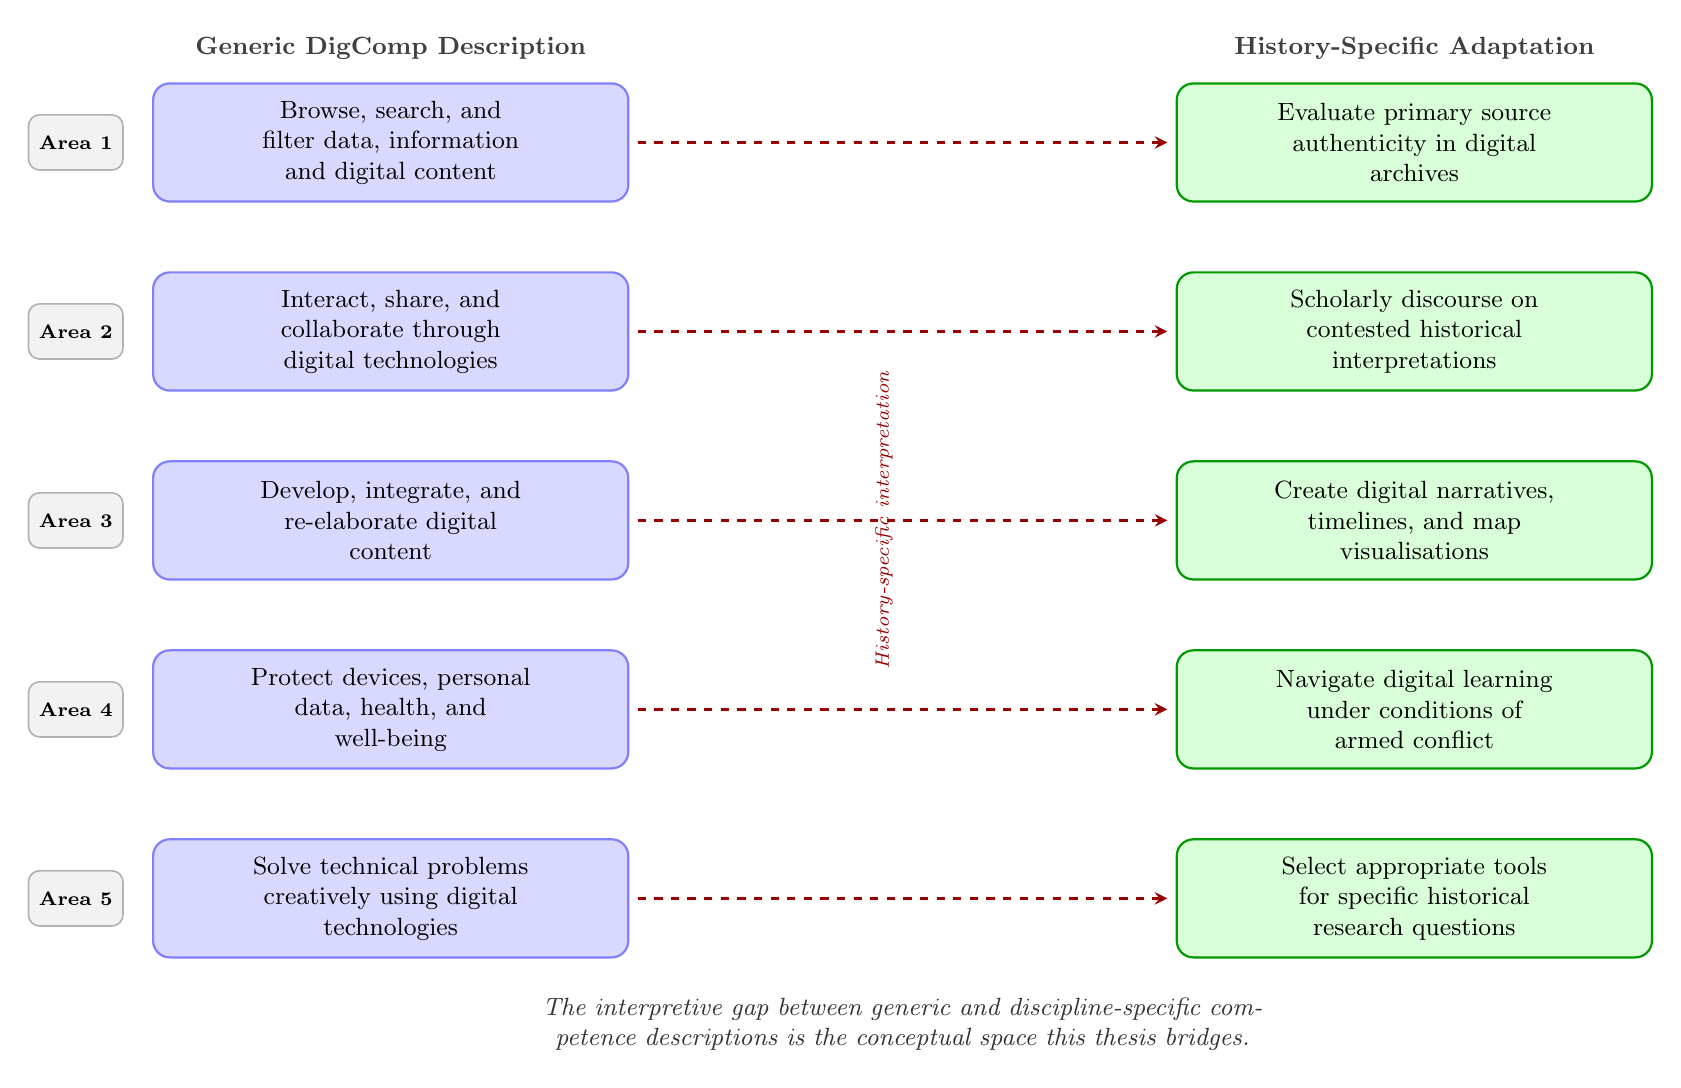
\begin{tikzpicture}[
  % Column styles
  generic/.style={rectangle, rounded corners=6pt, draw=blue!50, fill=blue!15,
    text width=5.8cm, minimum height=1.5cm, align=center, font=\small,
    line width=0.8pt},
  adapted/.style={rectangle, rounded corners=6pt, draw=green!60!black, fill=green!15,
    text width=5.8cm, minimum height=1.5cm, align=center, font=\small,
    line width=0.8pt},
  arealbl/.style={rectangle, rounded corners=4pt, draw=gray!60, fill=gray!10,
    minimum width=1.2cm, minimum height=0.7cm, align=center,
    font=\scriptsize\bfseries, line width=0.6pt},
  % Arrow style
  interp/.style={->, >=stealth, thick, draw=red!60!black, dashed, line width=1pt},
  % Annotation style
  note/.style={font=\small\itshape, text=gray!40!black, text width=14cm, align=center},
  % Header style
  header/.style={font=\small\bfseries\scshape, text=gray!50!black},
]

% Vertical spacing
\def\rowsep{2.4}
% Horizontal positions
\def\leftcol{-6.5}
\def\rightcol{6.5}
\def\arrowstart{-3.0}
\def\arrowend{3.0}
\def\arealblx{-10.5}

% Column headers
\node[header] at (\leftcol, 1.2) {Generic DigComp Description};
\node[header] at (0, 1.2) {};
\node[header] at (\rightcol, 1.2) {History-Specific Adaptation};

% --- Row 1: Information and data literacy ---
\node[arealbl] (a1) at (\arealblx, 0) {Area 1};
\node[generic] (g1) at (\leftcol, 0)
  {Browse, search, and\\filter data, information\\and digital content};
\node[adapted] (h1) at (\rightcol, 0)
  {Evaluate primary source\\authenticity in digital\\archives};
\draw[interp] ([xshift=3pt]g1.east) -- ([xshift=-3pt]h1.west);

% --- Row 2: Communication and collaboration ---
\node[arealbl] (a2) at (\arealblx, -\rowsep) {Area 2};
\node[generic] (g2) at (\leftcol, -\rowsep)
  {Interact, share, and\\collaborate through\\digital technologies};
\node[adapted] (h2) at (\rightcol, -\rowsep)
  {Scholarly discourse on\\contested historical\\interpretations};
\draw[interp] ([xshift=3pt]g2.east) -- ([xshift=-3pt]h2.west);

% --- Row 3: Digital content creation ---
\node[arealbl] (a3) at (\arealblx, -2*\rowsep) {Area 3};
\node[generic] (g3) at (\leftcol, -2*\rowsep)
  {Develop, integrate, and\\re-elaborate digital\\content};
\node[adapted] (h3) at (\rightcol, -2*\rowsep)
  {Create digital narratives,\\timelines, and map\\visualisations};
\draw[interp] ([xshift=3pt]g3.east) -- ([xshift=-3pt]h3.west);

% --- Row 4: Safety ---
\node[arealbl] (a4) at (\arealblx, -3*\rowsep) {Area 4};
\node[generic] (g4) at (\leftcol, -3*\rowsep)
  {Protect devices, personal\\data, health, and\\well-being};
\node[adapted] (h4) at (\rightcol, -3*\rowsep)
  {Navigate digital learning\\under conditions of\\armed conflict};
\draw[interp] ([xshift=3pt]g4.east) -- ([xshift=-3pt]h4.west);

% --- Row 5: Problem solving ---
\node[arealbl] (a5) at (\arealblx, -4*\rowsep) {Area 5};
\node[generic] (g5) at (\leftcol, -4*\rowsep)
  {Solve technical problems\\creatively using digital\\technologies};
\node[adapted] (h5) at (\rightcol, -4*\rowsep)
  {Select appropriate tools\\for specific historical\\research questions};
\draw[interp] ([xshift=3pt]g5.east) -- ([xshift=-3pt]h5.west);

% Central arrow label (placed once, vertically centred)
\node[font=\scriptsize\itshape, text=red!60!black, rotate=90, anchor=south]
  at (0, -2*\rowsep) {History-specific interpretation};

% Bottom annotation
\node[note] at (0, -4*\rowsep - 1.6)
  {The interpretive gap between generic and discipline-specific competence
   descriptions is the conceptual space this thesis bridges.};

\end{tikzpicture}%
}% end resizebox
\caption{History-specific interpretation of DigComp competence areas. Left: generic
descriptions from DigComp~2.0 \citep{Vuorikari2016}. Right: discipline-specific
adaptations developed in this thesis, grounded in the epistemological requirements
of historical inquiry \citep{Crymble2021, MonteSano2012} and the wartime
educational context \citep{UNESCO2023}. No existing literature provides such an
adaptation; this represents a contribution of the present study (see Section~\ref{sec:digcomp}).}
\label{fig:digcomp-history-adaptation}
\end{figure}
